\chapter{Orbital Optimization in Valence Bond Theory}
\label{chap_orbopt}

\ifthenelse{\boolean{wholethesis}}{\relax}{\begin{center}\textit{Generated on \today\ at \currenttime}\end{center}}

\noindent\textbf{Abstract:} The most time consuming step in optimizing a Valence Bond (VB) wave function with VBSCF is the construction of the matrix representation of the Hamilton operator ($\mathbf{H}$) and the corresponding overlap matrix ($\mathbf{S}$) for the wave function and the Brillouin states. In the 1990s a perturbation theory scheme, referred to as approximated Newton-Raphson (aNR), was introduced. For this scheme, less $\mathbf{H}$ matrix elements need to be constructed. In this chapter a further approximation is introduced. Instead of calculating $\mathbf{H}$ matrix elements the regular way, they are constructed from Fock matrix elements, taking less time.

\newpage

\section{Introduction}

\lettrine{\initial{I}}{}n 1916 Lewis suggested that atoms share electrons to form chemical bonds \cite{lewis}. Heitler and London incorporated this view a decade later into the quantum chemical description of the covalent bond in H$_2$ \cite{heitler}. In the 1930s Pauling used this description in his famous series of articles on ``The Nature Of The Chemical Bond'' \cite{pauling1,pauling2,pauling3,pauling4,pauling5,pauling6,pauling7,paulingbook}, which earned him the Nobel prize in 1954. This quantum chemical method is nowadays known as the Valence Bond theory.

In Valence Bond theory the wave function is more complex than in many other methods, like the Molecular Orbital theory \cite{hartree1,hartree2,hartree3,fock}. The VB orbitals have no orthogonality restriction and the wave function consists of multiple structures, consisting of one or more Slater determinants. Despite these computational hurdles, Valence Bond theory has kept a decent following through the years \cite{vboverv1,vboverv2,vboverv3}. One of the reasons is the development of powerful computers. On the other hand several efficient methods to optimize Valence Bond wave functions, Spin-Coupled Valence Bond (SCVB) \cite{scvb1,scvb2,scvb3}, Valence Bond Self-Consistent Field (VBSCF) \cite{vbscf1,vbscf2,koos1,zahid} and an algorithm that uses transition density matrices \cite{song}, have been developed.

Like a Valence Bond wave function, a Multi Configurational Self-Consistent Field (MCSCF) \cite{joop,mcscf,roos1,roos2} wave function is expressed in multiple structures, called Configuration State Functions (CSFs), comparable to VB structures. A peculiar difference, though, is the use of orthogonal orbitals in MCSCF. For the optimization of the orbitals in MCSCF, elements from a single Fock matrix are used to construct elements of the Hamiltonian matrix \cite{roos1}. The Fock matrix elements have the form:
\begin{equation}
F_{ia} = h_{ia} + \sum_{\sigma\nu} \left\{ \left[ \chi_i \chi_a | \chi_\sigma \chi_\nu \right] - \left[ \chi_i \chi_\nu | \chi_\sigma \chi_a \right] \right\} P^{(\sigma,\nu)},
\label{ch2.eq.fock}
\end{equation}
in which $F_{ia}$ is the Fock matrix element, $\chi_i$ and $\chi_a$ are spin-orbitals, $h_{ia}$ is the one electron integral $\left< \chi_i | \mathbf{h}| \chi_a \right>$. The double sum on the right hand side is over two electron integrals (Coulomb and exchange) times elements of the density matrix $P^{(\sigma,\nu)}$. 

This saves a substantial amount of computation time, because the Fock matrix needs does not depend on the expansion of the ground state wave function into the Super CI wave function \cite{superci1,superci2}. The central question for this chapter is whether it is also possible to use a single Fock matrix for the optimization of the orbitals in VBSCF, although those are non-orthogonal.

Song \textit{et al.} have shown that a VB wave function can be optimized with the help of transition density matrices from which multiple Fock matrices are constructed \cite{song}. The difference with the approach presented in this chapter is that here only a single Fock matrix is used that only depends on the number of determinants in the ground state wave function.

At first, the usability of Fock matrix elements in the Hamiltonian matrix is analyzed by comparing the expression for Fock matrix elements, equation \ref{ch2.eq.fock}, with the expression for Hamiltonian matrix elements by L\"{o}wdin \cite{lowdin}:
\begin{equation}
\left< \Delta_p | \hat{H} | \Delta_q \right> = \sum_{ik} h_{ik}S^{(i,k)} + \sum_{i<j,k<l} \left\{ \left[ \chi_i \chi_k | \chi_j \chi_l \right] - \left[ \chi_i \chi_l | \chi_j \chi_k \right] \right\}S^{(i,j,k,l)},
\label{ch2.eq.lowdindeterminants}
\end{equation}
where $\Delta_p$ and $\Delta_q$ are Slater determinants, $S^{(i,k)}$ and $S^{(i,j,k,l)}$ are first and second order cofactors and $h_{ik}$ and the term between curly brackets are one and two electron integrals, respectively.

The differences between equations \ref{ch2.eq.fock} and \ref{ch2.eq.lowdindeterminants} are in the summations. In the Fock matrix element, only a single one electron integral is present, while in L\"{o}wdins formula a double summation is found. For the two electron integrals, there is a double summation in the Fock matrix element, while  a quadruple summation appears in the formula of L\"{o}wdin. Besides, the Hamiltonian matrix element in equation \ref{ch2.eq.lowdindeterminants} is between two Slater determinants $\Delta_p$ and $\Delta_q$. Since VB wave functions consist of multiple determinants, a double summation over indexes $p$ and $q$ will be needed to compute a complete Hamiltonian matrix element. This double summation is absent in equation \ref{ch2.eq.fock}. 

Following the theoretical section, the implementation of these Fock matrix elements in TURTLE \cite{turtle}, the VB module in GAMESS-UK \cite{gamess}, will be presented. After the implementation details, speed-up factors of some test calculations will be discussed and compared. The chapter is concluded with an outlook on future enhancements.  

\section{Theory}

\subsection{\label{ch2.sec.vbsci}Valence Bond theory and Super CI}

To calculate the total energy of a molecular system, the time-independent Schr\"{o}dinger equation needs to be solved:
\begin{equation}
\mathbf{H}\Psi = E\Psi,
\end{equation}
in which $\mathbf{H}$ is the Hamilton operator, $\Psi$ is the wave function and $E$ is the total energy of the system. A wave function is said to be optimized once the lowest possible value $E$ has been found. For Valence Bond theory, such a wave function $\Psi$ is constructed from a linear combination of structures:
\begin{equation}
\Psi = \sum_{i} C_i \Phi_i.
\label{ch2.eq.vbwf}
\end{equation}
These structures are linear combinations of Slater determinants:
\begin{equation}
\Phi = \sum_{i} \gamma_i \Delta_i,
\label{ch2.eq.struct}
\end{equation}
which are antisymmetrized products of spin-orbitals:
\begin{equation}
\Delta = |\chi_i\chi_j\chi_k\chi_l \cdots \chi_n|,
\label{ch2.eq.determ}
\end{equation}
where the spin-orbitals $\chi$ have a spatial part and a spin part which can be $\alpha$ or $\beta$. Two examples are  $\chi_i(\mathbf{x})=\psi_i(\mathbf{r})\alpha(\omega)\equiv\psi_i$ and $\chi_j(\mathbf{x})=\psi_i(\mathbf{r})\beta(\omega)\equiv\overline{\psi_i}$.
Orbitals $\psi$ are linear combinations of one electron basis functions:
\begin{equation}
\psi = \sum_{n} c_n \phi_n,
\label{ch2.eq.basis}
\end{equation}
in which the $c_n$ are orbital coefficients and $\phi_n$ one electron basis functions.

A Valence Bond wave function can be optimized by modifying the structure coefficients $C_i$ (equation \ref{ch2.eq.vbwf}) and the orbital coefficients $c_n$ (equation \ref{ch2.eq.basis}). Both optimizations can be performed simultaneously, as is done in a Newton-Raphson scheme \cite{zahid}, or sequentially with a method like Super CI \cite{superci1,superci2}. In Super CI, the structure coefficients $C_i$ are calculated first by solving the secular equation:
\begin{equation}
[\mathbf{H}-E\mathbf{S}] \cdot \mathbf{C} = 0,
\label{ch2.eq.eig}
\end{equation}
in which $\mathbf{H}$ and $\mathbf{S}$ are the Hamiltonian and overlap matrix in structure basis, respectively. Secondly, the orbitals are optimized, as explained below. After the orbital optimization the secular equation \ref{ch2.eq.eig} is solved again with the new orbitals until both sets of coefficients no longer change.

Orbitals can be changed by adding a small amount of an other orbital. For instance, orbital $\psi_i$ can be changed by adding a small amount $\delta b_{ia}$ times $\psi_a$:
\begin{equation}
\psi_i' = \psi_i + \delta b_{ia} \psi_a.
\label{ch2.eq.orbchange}
\end{equation}
As a simple example, a single determinant wave function $\Psi_0=|\psi_i\overline{\psi_i}\psi_j\psi_k|$ with four orbitals is chosen. The orbitals $\psi_i$, $\psi_j$ and $\psi_k$ have $\alpha$ spin, while only $\overline{\psi_i}$ has $\beta$ spin. The orbital change of equation \ref{ch2.eq.orbchange} will result in:
\begin{equation}    
\begin{split}
|\psi_i'\overline{\psi_i'}\psi_j\psi_k | & = |(\psi_i + \delta b_{ia} \psi_a)\overline{(\psi_i + \delta b_{ia}\psi_a)}\psi_j\psi_k |\\
& = |\psi_i\overline{\psi_i}\psi_j\psi_k| + \delta b_{ia}|\psi_a\overline{\psi_i}\psi_j\psi_k| + \delta b_{ia} |\psi_i\overline{\psi_a}\psi_j\psi_k| + \delta b^2_{ia} |\psi_a\overline{\psi_a}\psi_j\psi_k|.\\
\end{split}
\label{ch2.eq.detchange}
\end{equation}
The first term is the original wave function $\Psi_0$. The second and third term are determinants, in which orbital $\psi_i$ has been replaced by $\psi_a$, once for $\alpha$ and once for $\beta$ spin. In the fourth determinant both occurrences of orbital $\psi_i$ have been replaced by $\psi_a$. This fourth determinant will be neglected here, because the amount $\delta b_{ia}$ is considered small and hence $\delta b_{ia}^2 \approx 0$.

The combination of the second and third determinant can be created from $|\psi_i\overline{\psi_i}\psi_j\psi_k |$ by the single excitation operator $\mathbf{C}_{i \rightarrow a}$, which replaces $\psi_i$ by $\psi_a$, once for $\alpha$ spin and once for $\beta$ spin \cite{ruttink}. This singly excited structure will be referred to as $\Psi_{ia}$. The change in $\Psi_0$ caused by the orbital change results (to first order) in:
\begin{equation}
\Psi_{0} \rightarrow \Psi_{0} + \delta b_{ia} \mathbf{C}_{i \rightarrow a} \Psi_{0} = \Psi_{0} + \delta b_{ia} \Psi_{ia}.
\label{ch2.eq.wfchange}
\end{equation}

With this mechanism orbital $\psi_i$ could be changed in such a way that the expectation value of the energy of $\Psi_0$ becomes lower. The minimum in the energy is found when the first order derivative of the energy with respect to the orbital change equals zero:
\begin{equation}
\frac{\partial E}{\partial b_{ia}}=\frac{\partial \frac{\left < \Psi_0 | \mathbf{H} | \Psi_0 \right >}{\left < \Psi_0 | \Psi_0 \right >}}{\partial b_{ia}}=0.
\label{ch2.eq.foderiv}
\end{equation}
Using the quotient rule, using the fact that $\left < \Psi_0 | \mathbf{H} | \Psi_0 \right >$ and $\left < \Psi_0 | \Psi_0 \right >$ are Hermitian and using that the first order derivative with respect to the orbital change of $\Psi_0$ in equation \ref{ch2.eq.wfchange} equals $\Psi_{ia}$ \cite{vbscf2}, the first order derivative of the energy with respect to the orbital change can be written as: 
\begin{equation}
\begin{split}
\frac{\partial E}{\partial b_{ia}} & = \frac{2 \cdot \left < \Psi_0 | \mathbf{H} | \Psi_{ia} \right > \left< \Psi_0 | \Psi_0 \right > - 2 \cdot \left < \Psi_0 | \mathbf{H} | \Psi_0  \right > \left< \Psi_0 | \Psi_{ia}\right>}{\left < \Psi_0 | \Psi_0 \right > ^2 }\\
& = \frac{ 2 \cdot \left < \Psi_0 | \mathbf{H} | \Psi_{ia} \right > - 2 \cdot E_0 \left< \Psi_0 | \Psi_{ia} \right >}{\left < \Psi_0 | \Psi_0 \right >}\\
& = \frac{ 2 \cdot \left < \Psi_0 | \mathbf{H} - E_0 | \Psi_{ia} \right >}{\left < \Psi_0 | \Psi_0 \right >}.
\end{split}
\label{ch2.eq.foderiv2}
\end{equation}
For optimal orbitals, this first order derivative is equal to zero and hence equation \ref{ch2.eq.foderiv2} reduces to:
\begin{equation}
\left < \Psi_0 | \mathbf{H} - E_0 | \Psi_{ia} \right > = 0,
\label{ch2.eq.brillouin}
\end{equation}
which is the Brillouin theorem \cite{brillouin,genbrill}. This theorem states that with optimal orbitals singly excited states ($\Psi_{ia}$) do not interact or mix with the reference or ground state ($\Psi_0$). 

In equations \ref{ch2.eq.orbchange}-\ref{ch2.eq.brillouin} the effect of a single orbital change has been shown. When all possible single excitations are taken into account, the wave function of equation \ref{ch2.eq.wfchange} can be written as:
\begin{equation}
\Psi_{superci} = \Psi_0 + \sum_{ia} b_{ia} \Psi_{ia},
\label{ch2.eq.superci}
\end{equation}
in which $\Psi_{superci}$ is the Super CI wave function, $i$ runs all orbitals from which an excitation can be performed and $a$ runs over all orbitals to which excitations can take place. Values for $b_{ia}$ can be found by solving the generalized eigenvalue problem:
\begin{equation}
[\mathbf{H}-E_b\mathbf{S}] \cdot \mathbf{b} = 0,
\label{ch2.eq.geig}
\end{equation}
in which $\mathbf{H}$ and $\mathbf{S}$ are the Hamiltonian and metric in the basis of singly excited states ($\Psi_0$ and the $\Psi_{ia}$'s). $E_b$ is the lowest eigenvalue and $\mathbf{b}$ is the corresponding eigenvector. With the elements of $\mathbf{b}$ the orbitals are updated to make $\Psi_0$ equal to $\Psi_{superci}$ to first order:
\begin{equation}
\psi_i' = \psi_i + \sum_{a} b_{ia} \psi_a.
\label{ch2.eq.orbupd}
\end{equation}
With the modification of the orbitals the Super CI wave function is contracted or condensed into $\Psi_0$. This is exemplified for the change in orbital $\psi_i$ in the simple one determinant wave function in equation \ref{ch2.eq.detchange}. Orbital $\psi_i$ in $\Psi_0$ is modified with $\delta b_{ia}$ times orbital $\psi_a$, which results in determinant $|\psi_i'\overline{\psi_i'}\psi_j\psi_k |$:
\begin{equation}
\begin{split}
\Psi_{0} \leftarrow & \Psi_{0} + \delta b_{ia} \Psi_{ia} = \\
&|\psi_i\overline{\psi_i}\psi_j\psi_k| + \delta b_{ia}(|\psi_a\overline{\psi_i}\psi_j\psi_k| + |\psi_i\overline{\psi_a}\psi_j\psi_k|) = \\
&|(\psi_i + \delta b_{ia}\psi_a)\overline{(\psi_i + \delta b_{ia}\psi_a)}\psi_j\psi_k| = \\
&|\psi_i'\overline{\psi_i'}\psi_j\psi_k |.\\
\end{split}
\label{ch2.eq.condense}
\end{equation}
So, $\Psi_0$ will contain the updated orbital $\psi_i'$ which will be denoted $\psi_i$ in the next step (iteration). This procedure for a single orbital update is performed for all combinations in the summation in the Super CI wave function. Since the orbital changes are performed independently, they may be counteracting and therefore the Brillouin condition may not be fulfilled in a single step. Therefore, a new excitation pattern for a new $\Psi_{superci}$ is created. The eigenvalue problem is solved again and the orbitals are updated once more. It is expected that the orbital updates become smaller with each step. This procedure is repeated until all Brillouin elements, $\left < \Psi_0 | \mathbf{H} - E_0 | \Psi_{ia} \right >$, have become zero. At that point the expectation value of the energy ($E_0$) is stationary with respect to orbital changes (equation \ref{ch2.eq.foderiv2}).

Up till here, $\Psi_0$ was constructed of a single determinant, \textit{i.e.} $|\psi_i\overline{\psi_i}\psi_j\psi_k|$. A regular VB wave function consists of multiple structures, and hence multiple determinants (see equations \ref{ch2.eq.vbwf} and \ref{ch2.eq.struct}). In that case, the contraction of equation \ref{ch2.eq.condense} will contain more determinants, all in which orbital $\psi_i$ has been replaced by $\psi_a$.

With the expansion into multiple determinants, three orbital classes can be distinguished. Firstly, orbitals that occur in all determinants, which will be denoted with subscripts $i$, $j$, $k$ and $l$. The second class contains orbitals that occur in some determinants, denoted with $t$, $u$, $v$ and $x$. The last class contains those orbitals that do not occur in the ground state wave function $\Psi_0$ and hence are virtual unoccupied orbitals $a$, $b$, $c$ and $d$.

To solve the generalized eigenvalue problem of equation \ref{ch2.eq.geig}, both the Hamiltonian ($\mathbf{H}$) and the overlap matrix ($\mathbf{S}$) are expressed in determinant form.  The Brillouin matrix is defined as the $\mathbf{H}$ matrix minus $E_0$ \cite{koos1}. Please note that for optimal orbitals, the Brillouin energy ($E_b$) in equation \ref{ch2.eq.geig} is equal to the energy of the ground state ($E_0$), because the singly exited states do no longer mix in with the ground state. 

An example of a Brillouin matrix, which contains elements resulting from two excitations: an excitation from $\psi_i$ to $\psi_a$ ($\Psi_{ia}$) and one from $\psi_i$ to $\psi_b$ ($\Psi_{ib}$), is shown below:
\begin{equation}
\left[\begin{array}{ccc}
\left< \Psi_{0} | \mathbf{H}-E_0 | \Psi_{0} \right> & \left< \Psi_{ia} | \mathbf{H}-E_0 | \Psi_{0} \right> & \left< \Psi_{ib} | \mathbf{H}-E_0 | \Psi_{0} \right> \\
\left< \Psi_{0} | \mathbf{H}-E_0 | \Psi_{ia} \right> & \left< \Psi_{ia} | \mathbf{H}-E_0 | \Psi_{ia} \right> & \left< \Psi_{ib} | \mathbf{H}-E_0 | \Psi_{ia} \right> \\
\left< \Psi_{0} | \mathbf{H}-E_0 | \Psi_{ib} \right> & \left< \Psi_{ia} | \mathbf{H}-E_0 | \Psi_{ib} \right> & \left< \Psi_{ib} | \mathbf{H}-E_0 | \Psi_{ib} \right> \\
\end{array}\right].
\label{ch2.eq.hamilt}
\end{equation}
The Brillouin matrix has the same dimension as the $\mathbf{H}$ and $\mathbf{S}$ matrices in equation \ref{ch2.eq.geig}. For each extra excitation the $\mathbf{H}$, $\mathbf{S}$ and Brillouin matrices are extended with one extra row and column. Hence, the number of elements increases roughly quadratic with the number of excitations.

The calculation of the elements in $\mathbf{H}$ is expensive because of the large number of determinants, caused by the expansion into the Super CI wave function: for each excitation a Brillouin state, containing 1 to 2 times the number of determinants of $\Psi_0$, is added. For each determinant combination the evaluation of (large amounts of) subdeterminants \cite{koos2}, or cofactors\footnote{Cofactors are described in detail in Appendix A.} are required.

To overcome this, van Lenthe \textit{et al.} presented a new method, referred to as approximated Newton-Raphson (Section \ref{ch2.sec.anr}), which requires less $\mathbf{H}$ and $\mathbf{S}$ matrix elements than regular Super CI \cite{koos1}, because elements of the type $\left < \Psi_{ia} | \mathbf{H} - E_0 | \Psi_{ib} \right >$ are not needed.

\subsection{\label{ch2.sec.anr}The Approximated Newton-Raphson Method}

In the approximated Newton-Raphson technique perturbation theory is used to obtain orbital update coefficients. These coefficients are approximated by the quotient of the first column element and the diagonal element on each row of equation \ref{ch2.eq.hamilt}:
\begin{equation}
b_{ia}= - \frac{\left< \Psi_{0} | \mathbf{H}-E_0 | \Psi_{ia} \right>}{\left< \Psi_{ia} | \mathbf{H}-E_0 | \Psi_{ia} \right>}.
\label{ch2.eq.anr}
\end{equation}
This means that elements of the type $\left< \Psi_{ia} | \mathbf{H}-E_0 | \Psi_{ib} \right>$ are not used. In that way, only two matrix elements need to be calculated for such an excitation, instead of $m$, where $m$ equals the total number of excitations. This reduces the quadratic increase in number of matrix elements to linear.

Although the update coefficients $b_{ia}$ are calculated in a different way, the total energy $E_0$ will be the same. Once the orbitals are optimal the numerator in equation \ref{ch2.eq.anr} becomes zero and hence the Brillouin condition is fulfilled. 

A further reduction of the calculation time can be achieved when the numerator and the denominator in equation \ref{ch2.eq.anr} could be calculated, or approximated, faster. As indicated in the introduction, the creation of a Fock matrix does not depend on the number of determinants in the wave function, while the Brillouin matrix elements in equation \ref{ch2.eq.anr} do. In the next section, the applicability of Fock matrix elements for the numerator and denominator in equation \ref{ch2.eq.anr} will be investigated.

\subsection{\label{ch2.sec.fock}Fock Matrix Elements} 

Roos \textit{et al.} showed that Brillouin matrix elements could be replaced by elements of the Fock matrix, based on the density matrix, for Complete Active Space Self-Consistent Field (CASSCF) wave functions \cite{roos1}. A CASSCF wave function is an MCSCF wave function for which all possible electron distributions in the variably occupied orbital space are included. They derived three different expressions with Fock matrix elements for three types of excitations:
\begin{itemize}
\item{$i \rightarrow a$ from (always) doubly occupied to virtual orbitals}
\item{$t \rightarrow a$ from variably occupied to virtual orbitals}
\item{$i \rightarrow t$ from (always) doubly to variably occupied orbitals}
\end{itemize}
The fourth type of excitation, $t \rightarrow t$ from variably to variably occupied orbitals, is not needed in CASSCF, because all possible electron distributions in the variably occupied orbital space are already included in $\Psi_0$. In this section all four types of excitations will be analyzed with L\"{o}wdins equation.

\subsubsection{\label{ch2.sec.i-a}$i \rightarrow a$ from (always) doubly to virtual orbitals}

The analysis of excitations of the type $i \rightarrow a$ is split into two parts. Firstly, the equality of the Brillouin matrix element with the Fock matrix is investigated for a single determinant wave function. After that, a wave function with multiple determinants is defined and analyzed.

The single determinant wave function has one doubly occupied orbital, $\phi_i$, being two spin-orbitals $\chi_i \equiv \phi_i$ and $\chi_j \equiv \overline{\phi_i}$. Furthermore, it has three variably occupied orbitals $\chi_t$, $\chi_u$ and $\chi_v$. Spin for these orbitals is not specified and hence no attention needs to be paid to the spin integration in the overlap matrices that follow. The ground state wave function $\Psi_0$ is then:
\begin{equation}
\Psi_0 = |\chi_i\chi_j\chi_t\chi_u\chi_v|.
\label{ch2.eq.wfexamp}
\end{equation}
Although not necessary, it is convenient to orthogonalize as many orbitals onto each other as possible \cite{vbscf2}. This results in the two occupied orbital subsets mentioned earlier, the always doubly occupied orbitals and the variably occupied orbitals. The remaining unoccupied orbitals are mostly chosen orthogonal to all other orbitals. For a detailed description of the construction of the virtual subspace, see the first appendix in reference \cite{koos1}. The overlap $\left < \Psi_0 | \Psi_0 \right>$ is the determinant of the overlap matrix:
\begin{equation}
\left < \Psi_0 | \Psi_0 \right> = | \mathbf{S} | =
\begin{array}{llllll}
 &  \chi_i & \chi_j & \chi_t & \chi_u & \chi_v \\
 \chi_i & \multicolumn{1}{|l}{ 1 } & 0 & 0 & 0 & \multicolumn{1}{l|}{ 0 } \\
 \chi_j & \multicolumn{1}{|l}{ 0 } & 1 & 0 & 0 & \multicolumn{1}{l|}{ 0 } \\
 \chi_t & \multicolumn{1}{|l}{ 0 } & 0 & 1 & s_{ut} & \multicolumn{1}{l|}{s_{vt}} \\
 \chi_u & \multicolumn{1}{|l}{ 0 } & 0 & s_{tu} & 1 & \multicolumn{1}{l|}{s_{vu}} \\
 \chi_v & \multicolumn{1}{|l}{ 0 } & 0 & s_{tv} & s_{uv} & \multicolumn{1}{l|}{1}
\end{array}.
\label{ch2.eq.s0}
\end{equation}

The density matrix, needed for the Fock matrix, is constructed from first order cofactors. An example of a density matrix element is $P^{(t,u)}$:
\begin{equation}
P^{(t,u)}=
\begin{array}{llllll}
 & \hskip 46.0 pt \hbox{\lower 93pt\hbox{\vrule height100pt width 1.0pt}}\hskip-47.0pt \chi_i & \chi_j & \chi_t & \chi_u & \chi_v \\
 \noalign{\vskip-91pt}
 \chi_i &  \multicolumn{1}{|l}{ 1 } & 0 & 0 & 0 & \multicolumn{1}{l|}{ 0 } \\
 \chi_j & \multicolumn{1}{|l}{ 0 } & 1 & 0 & 0 & \multicolumn{1}{l|}{ 0 } \\
 \chi_t & \multicolumn{1}{|l}{ 0 } & 0 & 1 & s_{ut} & \multicolumn{1}{l|}{s_{vt}} \\
 \chi_u & \multicolumn{1}{|l}{ 0 } & 0 & s_{tu} & 1 & \multicolumn{1}{l|}{s_{vu}} \\
 \noalign{\vskip-8pt}
 \multispan6\hbox{\vrule  height 1.0 pt width130pt}\cr
 \noalign{\vskip 7pt}
 \chi_v & \multicolumn{1}{|l}{ 0 } & 0 & s_{tv} & s_{uv} & \multicolumn{1}{l|}{ 1 }
\end{array} =
\begin{array}{lllll}
 &  \chi_i & \chi_j & \chi_u & \chi_v \\
 \chi_i & \multicolumn{1}{|l}{ 1 } & 0 & 0 & \multicolumn{1}{l|}{ 0 } \\
 \chi_j & \multicolumn{1}{|l}{ 0 } & 1 & 0 & \multicolumn{1}{l|}{ 0 } \\
 \chi_t & \multicolumn{1}{|l}{ 0 } & 0 & s_{ut} & \multicolumn{1}{l|}{s_{vt}} \\
 \chi_v & \multicolumn{1}{|l}{ 0 } & 0 & s_{uv} & \multicolumn{1}{l|}{1}
\end{array},
\label{ch2.eq.p0examp}
\end{equation}
which is a cofactor, or subdeterminant of the overlap matrix.

Since $\psi_i$ is doubly occupied, in $\chi_i$ and $\chi_j$, there are also two virtual orbitals for $\psi_a$, being $\chi_a \equiv \psi_a$ and $\chi_b \equiv \overline{\psi_a}$. The singly excited state wave function is $\Psi_{ia} = |\chi_a\chi_j\chi_t\chi_u\chi_v| + |\chi_i\chi_b\chi_t\chi_u\chi_v|$. These determinants will be referred to as $\Delta_{ia}$ and $\Delta_{jb}$, respectively. The overlap between $\Psi_0$, denoted here as $\Delta_0$, and both these determinants is:
\begin{equation}
\left < \Delta_0 | \Delta_{ia} \right > = 
\begin{array}{llllll}
 &  \chi_i & \chi_j & \chi_t & \chi_u & \chi_v \\
 \chi_a & \multicolumn{1}{|l}{ 0 } & 0 & 0 & 0 & \multicolumn{1}{l|}{ 0 } \\
 \chi_j & \multicolumn{1}{|l}{ 0 } & 1 & 0 & 0 & \multicolumn{1}{l|}{ 0 } \\
 \chi_t & \multicolumn{1}{|l}{ 0 } & 0 & 1 & s_{ut} & \multicolumn{1}{l|}{s_{vt}} \\
 \chi_u & \multicolumn{1}{|l}{ 0 } & 0 & s_{tu} & 1 & \multicolumn{1}{l|}{s_{vu}} \\
 \chi_v & \multicolumn{1}{|l}{ 0 } & 0 & s_{tv} & s_{uv} & \multicolumn{1}{l|}{1}
\end{array}
\label{ch2.eq.psi0_ia}
\end{equation}
and
\begin{equation}
\left < \Delta_0 | \Delta_{jb} \right > = 
\begin{array}{llllll}
 &  \chi_i & \chi_j & \chi_t & \chi_u & \chi_v \\
 \chi_i & \multicolumn{1}{|l}{ 1 } & 0 & 0 & 0 & \multicolumn{1}{l|}{ 0 } \\
 \chi_b & \multicolumn{1}{|l}{ 0 } & 0 & 0 & 0 & \multicolumn{1}{l|}{ 0 } \\
 \chi_t & \multicolumn{1}{|l}{ 0 } & 0 & 1 & s_{ut} & \multicolumn{1}{l|}{s_{vt}} \\
 \chi_u & \multicolumn{1}{|l}{ 0 } & 0 & s_{tu} & 1 & \multicolumn{1}{l|}{s_{vu}} \\
 \chi_v & \multicolumn{1}{|l}{ 0 } & 0 & s_{tv} & s_{uv} & \multicolumn{1}{l|}{1}
\end{array},
\label{ch2.eq.psi0_jb}
\end{equation}
which are both zero, because they contain a row and a column with zeroes.

To construct the Brillouin matrix element (equation \ref{ch2.eq.lowdindeterminants}), first and second order cofactors from the determinants in equations \ref{ch2.eq.psi0_ia} and \ref{ch2.eq.psi0_jb} are needed. Only two first order cofactors have a non zero value, $S^{(i,a)}$ created by removing column $\chi_i$ and row $\chi_a$ from the determinant in equation \ref{ch2.eq.psi0_ia} and $S^{(j,b)}$ created by removing column $\chi_j$ and row $\chi_b$ from the determinant in equation \ref{ch2.eq.psi0_jb}. Other first order cofactors will be zero, because removing any other row or column will lead to a row or column with zeroes.

This means that per determinant combination only a single one electron integral contributes to the Brillouin matrix element, \textit{i.e.} $h_{ia} \cdot S^{(i,a)}$ and $h_{jb} \cdot S^{(j,b)}$. While the spin parts in $h_{ia}$ and $h_{jb}$ differ, $\chi_i$ and $\chi_a$ have $\alpha$ spin and $\chi_j$ and $\chi_b$ have $\beta$ spin, their spatial parts are equal. Furthermore, the first order cofactors, $S^{(i,a)}$ and $S^{(j,b)}$, and the overlap determinant (equation \ref{ch2.eq.s0}) differ one unit in rank. The overlap determinant has a single ``1'' on the diagonal of the extra row and column and hence these cofactors are equal to the overlap:
\begin{equation}
|\mathbf{S}| =
\begin{array}{llllll}
 &  \chi_i & \chi_j & \chi_t & \chi_u & \chi_v \\
 \chi_i & \multicolumn{1}{|l}{ 1 } & 0 & 0 & 0 & \multicolumn{1}{l|}{ 0 } \\
 \chi_j & \multicolumn{1}{|l}{ 0 } & 1 & 0 & 0 & \multicolumn{1}{l|}{ 0 } \\
 \chi_t & \multicolumn{1}{|l}{ 0 } & 0 & 1 & s_{ut} & \multicolumn{1}{l|}{s_{vt}} \\
 \chi_u & \multicolumn{1}{|l}{ 0 } & 0 & s_{tu} & 1 & \multicolumn{1}{l|}{s_{vu}} \\
 \chi_v & \multicolumn{1}{|l}{ 0 } & 0 & s_{tv} & s_{uv} & \multicolumn{1}{l|}{1}
\end{array}=
\begin{array}{lllll}
 &  \chi_j & \chi_t & \chi_u & \chi_v \\
 \chi_j & \multicolumn{1}{|l}{ 1 } & 0 & 0 & \multicolumn{1}{l|}{ 0 } \\
 \chi_t & \multicolumn{1}{|l}{ 0 } & 1 & s_{ut} & \multicolumn{1}{l|}{ s_{vt} } \\
 \chi_u & \multicolumn{1}{|l}{ 0 } & s_{tu} & 1 & \multicolumn{1}{l|}{s_{vu}} \\
 \chi_v & \multicolumn{1}{|l}{ 0 } & s_{tv} & s_{uv} & \multicolumn{1}{l|}{1}
\end{array}=
S^{(i,a)},
\label{ch2.eq.sissia}
\end{equation}
and
\begin{equation}
S^{(i,a)}=
\begin{array}{lllll}
 &  \chi_j & \chi_t & \chi_u & \chi_v \\
 \chi_j & \multicolumn{1}{|l}{ 1 } & 0 & 0 & \multicolumn{1}{l|}{ 0 } \\
 \chi_t & \multicolumn{1}{|l}{ 0 } & 1 & s_{ut} & \multicolumn{1}{l|}{ s_{vt} } \\
 \chi_u & \multicolumn{1}{|l}{ 0 } & s_{tu} & 1 & \multicolumn{1}{l|}{s_{vu}} \\
 \chi_v & \multicolumn{1}{|l}{ 0 } & s_{tv} & s_{uv} & \multicolumn{1}{l|}{1}
\end{array}=
\begin{array}{lllll}
 &  \chi_i & \chi_t & \chi_u & \chi_v \\
 \chi_i & \multicolumn{1}{|l}{ 1 } & 0 & 0 & \multicolumn{1}{l|}{ 0 } \\
 \chi_t & \multicolumn{1}{|l}{ 0 } & 1 & s_{ut} & \multicolumn{1}{l|}{ s_{vt} } \\
 \chi_u & \multicolumn{1}{|l}{ 0 } & s_{tu} & 1 & \multicolumn{1}{l|}{s_{vu}} \\
 \chi_v & \multicolumn{1}{|l}{ 0 } & s_{tv} & s_{uv} & \multicolumn{1}{l|}{1}
\end{array}=
S^{(j,b)}.
\end{equation}
Since the wave function $\Psi_0$ is normalized, its overlap is one. Therefore, $S^{(i,a)}$ and $S^{(j,b)}$ are also one and with it the one electron contribution to the Brillouin matrix element reduces to $2 \cdot h_{ia}$.

The two electron integrals in equation \ref{ch2.eq.lowdindeterminants} are multiplied by second order cofactors. This means that besides removing column $\chi_i$ and row $\chi_a$ from the determinant in equation \ref{ch2.eq.psi0_ia} and column $\chi_j$ and row $\chi_b$ from the determinant in equation \ref{ch2.eq.psi0_jb}, another row and column need to be removed to create these second order cofactors. Since index $i$ and $a$ (equation \ref{ch2.eq.psi0_ia}) and $j$ and $b$ (equation \ref{ch2.eq.psi0_jb}) are fixed, the summation in the two electron integral part of equation \ref{ch2.eq.lowdindeterminants} will only run over the other two indexes $\sigma$ and $\nu$:
\begin{equation}
\sum_{\sigma\nu} \left\{ [\chi_i\chi_a|\chi_\sigma\chi_\nu] - [\chi_i\chi_\nu|\chi_\sigma\chi_a] \right\} S^{(i,\sigma,a,\nu)}
\label{ch2.eq.twoel_ia}
\end{equation}
and
\begin{equation}
\sum_{\sigma\nu} \left\{ [\chi_j\chi_b|\chi_\sigma\chi_\nu] - [\chi_j\chi_\nu|\chi_\sigma\chi_b] \right\} S^{(j,\sigma,b,\nu)}
\label{ch2.eq.twoel_jb}
\end{equation}
Because the operator in the two electron integral part, $\frac{1}{r_{12}}$, only operates on the spatial coordinates, the expressions in equations \ref{ch2.eq.twoel_ia} and \ref{ch2.eq.twoel_jb} are the same. Furthermore, second order cofactors $S^{(i,\sigma,a,\nu)}$ are equal to density matrix elements $P^{(\sigma,\nu)}$ (equation \ref{ch2.eq.p0examp}). The rank of a density matrix element is one higher than that of a second order cofactor. Like in the one electron part case, this extra rank has a ``1'' on the diagonal, while the rest of its column and row are zero. An example is the previously mentioned $P^{(t,u)}$ (equation \ref{ch2.eq.p0examp}) which is equal to $S^{(i,t,a,u)}$:
\begin{equation}
P^{(t,u)}=
\begin{array}{lllll}
 &  \chi_i & \chi_j & \chi_u & \chi_v \\
 \chi_i & \multicolumn{1}{|l}{ 1 } & 0 & 0 & \multicolumn{1}{l|}{ 0 } \\
 \chi_j & \multicolumn{1}{|l}{ 0 } & 1 & 0 & \multicolumn{1}{l|}{ 0 } \\
 \chi_t & \multicolumn{1}{|l}{ 0 } & 0 & s_{ut} & \multicolumn{1}{l|}{s_{vt}} \\
 \chi_v & \multicolumn{1}{|l}{ 0 } & 0 & s_{uv} & \multicolumn{1}{l|}{1}
\end{array}=
\begin{array}{llll}
 & \chi_j & \chi_u & \chi_v \\
 \chi_j & \multicolumn{1}{|l}{ 1 } & 0 & \multicolumn{1}{l|}{ 0 } \\
 \chi_t & \multicolumn{1}{|l}{ 0 } & s_{ut} & \multicolumn{1}{l|}{s_{vt}} \\
 \chi_v & \multicolumn{1}{|l}{ 0 } & s_{uv} & \multicolumn{1}{l|}{1}
\end{array}=S^{(i,t,a,u)}.
\end{equation}
With this, the total two electron integral contribution reduces to:
\begin{equation}
2 \cdot \sum_{\sigma\nu} \left\{ [\chi_i\chi_a|\chi_\sigma\chi_\nu] - [\chi_i\chi_\nu|\chi_\sigma\chi_a] \right\} P^{(\sigma,\nu)}.
\label{ch2.eq.twoel_ia_tot}
\end{equation}
Therefore, the total Brillouin matrix element is:
\begin{equation}
\begin{split}
\left < \Psi_0 | \hat{H} | \Psi_{ia} \right > & = 2 \cdot ( h_{ia} + \sum_{\sigma\nu} \left\{ [\chi_i\chi_a|\chi_\sigma\chi_\nu] - [\chi_i\chi_\nu|\chi_\sigma\chi_a] \right\} P^{(\sigma,\nu)}) \\
& = 2 \cdot F_{ia}.
\end{split}
\end{equation}

Up till here only a single determinant wave function was used. A VB wave function consists of any number of determinants and therefore the derivation above will be expanded to multiple determinants. A new VB wave function, consisting of one doubly occupied orbital $\psi_i$, expressed in spin-orbitals $\chi_i$ and $\chi_j$, and four partly occupied orbital, $\chi_t$, $\chi_u$, $\chi_v$ and $\chi_x$, is defined:
\begin{equation}
\Psi_0 = |\chi_i\chi_j\chi_t\chi_u|+|\chi_i\chi_j\chi_v\chi_x|.
\label{ch2.eq.wfexamp2}
\end{equation}
The corresponding overlap determinant $|\mathbf{S}| = \left< \Psi_0 | \Psi_0 \right>$ is:
\begin{equation}
\begin{split}
|\mathbf{S}|=&
\begin{array}{lllll}
 &  \chi_i & \chi_j & \chi_t & \chi_u \\
 \chi_i & \multicolumn{1}{|l}{ 1 } & 0 & 0 & \multicolumn{1}{l|}{ 0 } \\
 \chi_j & \multicolumn{1}{|l}{ 0 } & 1 & 0 & \multicolumn{1}{l|}{ 0 } \\
 \chi_t & \multicolumn{1}{|l}{ 0 } & 0 & 1 & \multicolumn{1}{l|}{s_{ut}} \\
 \chi_u & \multicolumn{1}{|l}{ 0 } & 0 & s_{tu} & \multicolumn{1}{l|}{1}
\end{array}+
\begin{array}{lllll}
 &  \chi_i & \chi_j & \chi_t & \chi_u \\
 \chi_i & \multicolumn{1}{|l}{ 1 } & 0 & 0 & \multicolumn{1}{l|}{ 0 } \\
 \chi_j & \multicolumn{1}{|l}{ 0 } & 1 & 0 & \multicolumn{1}{l|}{ 0 } \\
 \chi_v & \multicolumn{1}{|l}{ 0 } & 0 & s_{tv} & \multicolumn{1}{l|}{s_{uv}} \\
 \chi_x & \multicolumn{1}{|l}{ 0 } & 0 & s_{tx} & \multicolumn{1}{l|}{s_{ux}}
\end{array} \\
& + \begin{array}{lllll}
 &  \chi_i & \chi_j & \chi_v & \chi_x \\
 \chi_i & \multicolumn{1}{|l}{ 1 } & 0 & 0 & \multicolumn{1}{l|}{ 0 } \\
 \chi_j & \multicolumn{1}{|l}{ 0 } & 1 & 0 & \multicolumn{1}{l|}{ 0 } \\
 \chi_t & \multicolumn{1}{|l}{ 0 } & 0 & s_{vt} & \multicolumn{1}{l|}{s_{xt}} \\
 \chi_u & \multicolumn{1}{|l}{ 0 } & 0 & s_{vu} & \multicolumn{1}{l|}{s_{xu}}
\end{array}+
\begin{array}{lllll}
 &  \chi_i & \chi_j & \chi_v & \chi_x \\
 \chi_i & \multicolumn{1}{|l}{ 1 } & 0 & 0 & \multicolumn{1}{l|}{ 0 } \\
 \chi_j & \multicolumn{1}{|l}{ 0 } & 1 & 0 & \multicolumn{1}{l|}{ 0 } \\
 \chi_v & \multicolumn{1}{|l}{ 0 } & 0 & 1 & \multicolumn{1}{l|}{s_{xv}} \\
 \chi_x & \multicolumn{1}{|l}{ 0 } & 0 & s_{vx} & \multicolumn{1}{l|}{ 1 }
\end{array}.
\end{split}
\label{ch2.eq.s02}
\end{equation}

The density matrix is constructed by looping through the determinants in equation \ref{ch2.eq.s02} and if the row and column index of the density matrix element are present in the determinant, a cofactor is created and added to the density matrix element. Since orbitals $\chi_i$ and $\chi_j$ occur in all determinants, density matrix elements $P^{(i,i)}$ and $P^{(j,j)}$ get a contribution from cofactors of all these determinants. Other elements get a contribution from less determinants, a single one in this case. For example, $P^{(t,x)}$ is:
\begin{equation}
P^{(t,x)}=
\begin{array}{llll}
 &  \chi_i & \chi_j & \chi_u \\
 \chi_i & \multicolumn{1}{|l}{ 1 } & 0 & \multicolumn{1}{l|}{ 0 } \\
 \chi_j & \multicolumn{1}{|l}{ 0 } & 1 & \multicolumn{1}{l|}{ 0 } \\
 \chi_v & \multicolumn{1}{|l}{ 0 } & 0 & \multicolumn{1}{l|}{ s_{uv} }
\end{array}.
\label{ch2.eq.p0examp2}
\end{equation} 

In the one determinant case it has been shown that the procedure for $\alpha$ and $\beta$ spin is the same. Therefore, only the excitation for the $\alpha$ spin electron will be analyzed. The overlap of $\Psi_0$ with $\Psi_{ia}$ is:
\begin{equation}
\begin{split}
\left<\Psi_0|\Psi_{ia} \right> =&
\begin{array}{lllll}
 &  \chi_i & \chi_j & \chi_t & \chi_u \\
 \chi_a & \multicolumn{1}{|l}{ 0 } & 0 & 0 & \multicolumn{1}{l|}{ 0 } \\
 \chi_j & \multicolumn{1}{|l}{ 0 } & 1 & 0 & \multicolumn{1}{l|}{ 0 } \\
 \chi_t & \multicolumn{1}{|l}{ 0 } & 0 & 1 & \multicolumn{1}{l|}{s_{ut}} \\
 \chi_u & \multicolumn{1}{|l}{ 0 } & 0 & s_{tu} & \multicolumn{1}{l|}{1}
\end{array}+
\begin{array}{lllll}
 &  \chi_i & \chi_j & \chi_t & \chi_u \\
 \chi_a & \multicolumn{1}{|l}{ 0 } & 0 & 0 & \multicolumn{1}{l|}{ 0 } \\
 \chi_j & \multicolumn{1}{|l}{ 0 } & 1 & 0 & \multicolumn{1}{l|}{ 0 } \\
 \chi_v & \multicolumn{1}{|l}{ 0 } & 0 & s_{tv} & \multicolumn{1}{l|}{s_{uv}} \\
 \chi_x & \multicolumn{1}{|l}{ 0 } & 0 & s_{tx} & \multicolumn{1}{l|}{s_{ux}}
\end{array} \\
& +\begin{array}{lllll}
 &  \chi_i & \chi_j & \chi_v & \chi_x \\
 \chi_a & \multicolumn{1}{|l}{ 0 } & 0 & 0 & \multicolumn{1}{l|}{ 0 } \\
 \chi_j & \multicolumn{1}{|l}{ 0 } & 1 & 0 & \multicolumn{1}{l|}{ 0 } \\
 \chi_t & \multicolumn{1}{|l}{ 0 } & 0 & s_{vt} & \multicolumn{1}{l|}{s_{xt}} \\
 \chi_u & \multicolumn{1}{|l}{ 0 } & 0 & s_{vu} & \multicolumn{1}{l|}{s_{xu}}
\end{array}+
\begin{array}{lllll}
 &  \chi_i & \chi_j & \chi_v & \chi_x \\
 \chi_a & \multicolumn{1}{|l}{ 0 } & 0 & 0 & \multicolumn{1}{l|}{ 0 } \\
 \chi_j & \multicolumn{1}{|l}{ 0 } & 1 & 0 & \multicolumn{1}{l|}{ 0 } \\
 \chi_v & \multicolumn{1}{|l}{ 0 } & 0 & 1 & \multicolumn{1}{l|}{s_{xv}} \\
 \chi_x & \multicolumn{1}{|l}{ 0 } & 0 & s_{vx} & \multicolumn{1}{l|}{ 1 }
\end{array}.
\end{split}
\label{ch2.eq.psi0_ia2}
\end{equation}
The only one electron contribution that adds to the Brillouin matrix element is $h_{ia}$, because it is multiplied by non zero  cofactors created by removing column $\chi_i$ and row $\chi_a$ from all four determinants in equation \ref{ch2.eq.psi0_ia2}. The sum of these four cofactors is equal to the sum in equation \ref{ch2.eq.s02}. Since $\Psi_0$ is normalized, this is equal to one. The contribution is then, like for the one determinant case, $h_{ia}$ for $\alpha$ spin.

Only those two electron integrals that contain second order cofactors in which column $\chi_i$ and row $\chi_a$ are removed occur. One such a two electron integral that contributes is: 
\begin{equation}
\left\{ [\chi_i\chi_a|\chi_t\chi_x] - [\chi_i\chi_x|\chi_t\chi_a] \right\} S^{(i,t,a,x)},
\label{ch2.eq.twoelexamp2}
\end{equation}
in which
\begin{equation}
S^{(i,t,a,x)}= 
\begin{array}{lll}
 &  \chi_j & \chi_u \\
 \chi_j & \multicolumn{1}{|l}{ 1 } & \multicolumn{1}{l|}{ 0 } \\
 \chi_v & \multicolumn{1}{|l}{ 0 } & \multicolumn{1}{l|}{ s_{uv} }
\end{array}=
\begin{array}{llll}
 &  \chi_i & \chi_j & \chi_u \\
 \chi_i & \multicolumn{1}{|l}{ 1 } & 0 & \multicolumn{1}{l|}{ 0 } \\
 \chi_j & \multicolumn{1}{|l}{ 0 } & 1 & \multicolumn{1}{l|}{ 0 } \\
 \chi_v & \multicolumn{1}{|l}{ 0 } & 0 & \multicolumn{1}{l|}{ s_{uv} }
\end{array}=
P^{(t,x)}
\label{ch2.eq.cofac2isp2}
\end{equation}

\subsubsection{\label{ch2.sec.t-a}$t \rightarrow a$ from variably occupied to virtual orbitals}



\subsubsection{\label{ch2.sec.denominator}Approximation Of The Denominator}

As stated before, the numerator in equation \ref{ch2.eq.anr} is needed to check whether the minimum in the energy is reached and therefore the Fock matrix element has got to be equal to the Brillouin matrix element. For the denominator, there is no such hard condition, since it is only used as weighting factor. 

The diagonal element in the Brillouin matrix is:
\begin{equation}
\left< \Psi_{ia} | \mathbf{H}-E_0 | \Psi_{ia} \right>  =  \left< \Psi_{ia} | \mathbf{H} | \Psi_{ia} \right>  - E_0 \left< \Psi_{ia} | \Psi_{ia} \right>.
\label{ch2.eq.brildiag}
\end{equation}
The difference between $\left < \Psi_{ia} | \mathbf{H} | \Psi_{ia} \right >$ and $E_0 \left< \Psi_{ia} | \Psi_{ia} \right>$ can be approximated with the help of Fock matrix elements on the diagonal:
the expectation value of the energy of the excited state ($\left< \Psi_{ia} | \mathbf{H} | \Psi_{ia} \right>$) is roughly the ground state energy ($E_0$, $\Psi_{ia}$ is not normalized: part of the approximation) minus the energy of the no longer occupied orbital $i$ (roughly $F_{ii}$) plus the energy of the newly occupied $a$ (roughly $F_{aa}$). The denominator then becomes:
\begin{equation}
\frac{\left< \Psi_{ia} | \mathbf{H}-E_0 | \Psi_{ia} \right>}{\left< \Psi_{ia} | \Psi_{ia} \right>} \approx (F_{aa}-F_{ii}).
\label{ch2.eq.cheapdiag}
\end{equation}
This is an approximation, since removing an orbital will influence other orbitals, which is not taken into account here. This approximation may or may not work. An advantage of approximating the diagonal Brillouin matrix element with the difference of two Fock matrix elements is that it saves time, especially when the wave function consists of a lot of determinants. On the other hand, since it is an approximation it might result in more iterations. This means that in some situations/calculations it will speed up, while in others it won't.

\section{\label{ch2.sec.implementation}Implementation}

The implementation of the approximations described in the previous section consists of two parts. Firstly, the approximated Newton-Raphson method, which was already implemented in TURTLE, has been extended with extra options. Secondly, the use of a Fock matrix for the optimization of doubly occupied orbitals has been implemented from scratch.

In the original aNR implementation the perturbation (equation \ref{ch2.eq.anr}) was used for excitations from the always and partly occupied orbitals to the virtuals. For all other excitations, \textit{i.e.} those from the always occupied orbitals to the partly occupied orbitals and from partly occupied to other partly occupied orbitals, an $\mathbf{H}$ and $\mathbf{S}$ matrix were constructed, for which the update coefficients were retrieved by solving the generalized eigenvalue problem (equation \ref{ch2.eq.geig}). 

In the current implementation there are three optimization options per excitation. The first option is that the excitation is treated with Super CI. In that case all interaction elements will be calculated. These are the interaction element of the ground state with the singly excited state, like $\left < \Psi_{0} | \mathbf{H} - E_0 | \Psi_{ia} \right >$, the diagonal element, $\left < \Psi_{ia} | \mathbf{H} - E_0 | \Psi_{ia} \right >$, and all interaction elements with other singly excited structures, like $\left < \Psi_{ia} | \mathbf{H} - E_0 | \Psi_{ib} \right >$. Please note, that these latter elements are only calculated when both excitations ($i \rightarrow a$ and $i \rightarrow b$) are treated with Super CI.

The second option is that the excitation is treated with approximated Newton-Raphson. In that case only the two matrix elements in equation \ref{ch2.eq.anr} are calculated to obtain the update coefficient $b_{ia}$.

In the third option the excitation is treated with the Fock operator. In that case the orbital update coefficient $b_{ia}$ is calculated by dividing the Fock matrix element of the type $F_{ia}$ by the difference between $F_{ii}$ and $F_{aa}$ (Section \ref{ch2.sec.denominator}):
\begin{equation}
b_{ia}= - \frac{F_{ia}}{F_{aa}-F_{ii}}.
\label{ch2.eq.fockapprox}
\end{equation}

For excitations treated with regular Super CI, the $\mathbf{b}$ vector is calculated by solving the generalized eigenvalue problem (equation \ref{ch2.eq.geig}). This eigenvector is then padded with the separately calculated update coefficients of equations \ref{ch2.eq.anr} and \ref{ch2.eq.fockapprox}. With the elements from of this $\mathbf{b}$ vector the orbitals are updated, like in equation \ref{ch2.eq.condense}.

The three options above suggest that the user needs to specify beforehand which Brillouin matrix rows (or excitations) should be treated with which option. Since the virtual space is not yet created at the beginning of the calculation it is not very practical to specify the optimization method per excitation. Therefore, two additional specification options have been added: the specification per occupied orbital and the specification per orbital class. All excitations for either a certain orbital or all orbitals in a class are treated with the same option, be-it \textit{superci}, \textit{pert} or \textit{fock}. There are three orbital classes: doubly occupied (doc), variably occupied (voc) and unoccupied (uoc). The doubly occupied class contains orbitals that occur twice in each determinant, once with $\alpha$ and once with $\beta$ spin. The variably occupied class contains orbitals which occur in some determinants and the unoccupied orbital class contains orbitals which only occur in excited state structures. It should be noted that the \textit{fock} option can only be used for the optimization of orbitals which are orthogonal to all other orbitals. The most commonly used specification option, at least for the calculations reported in this thesis, is the specification per orbital class. 

\section{Sample Calculations}

In this section results from a few test calculations will be presented. In the first example some of the new parameters for the extended \textit{pert} option are tested. The results are compared to those from a complete Super CI calculation. In the second example results from several calculations with the \textit{superci}, the \textit{pert} and the new \textit{fock} option are compared.  

\subsection{\label{ch2.sec.cyclopent}First Example: The Cp-SiH Molecule}

For the work described in Chapter \chcyclopentadienyl\ a number of local VBSCF calculations have been performed to investigate the bonding mechanism of main group metal hydrides to cyclopentadienyl moieties. For details on the geometry optimization and the basis sets used, see Chapter \chcyclopentadienyl\ and reference \cite{budzelaar}. One of the molecules from that research is taken, the $\sigma$ bound \mbox{Cp-SiH} structure (Figure \ref{fig.cpsih}).
\begin{figure}[htdp]
\center
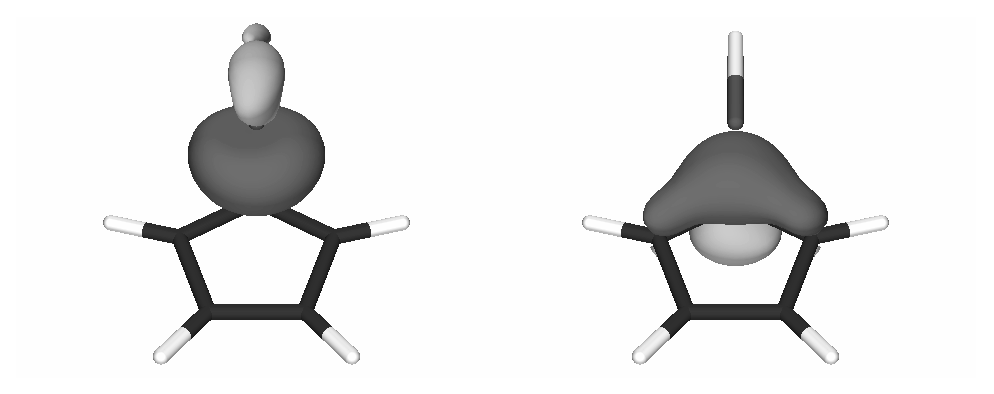
\includegraphics[scale=0.6]{orbopt/figures/sigma_sih.eps}
\caption{The $\sigma$ bound structure of Cp-SiH. Shown are the two singly occupied orbitals: the $sp$ hybridized orbital on SiH (left) and a $p$ orbital on the Cp-ring (right).}
\label{fig.cpsih}
\end{figure}
The calculation on this molecule forms a useful example for testing the additions to the optimization options, because the VBSCF process changes the orbitals drastically (in this case the total energy drops 0.86 Hartree between the initial and the final iteration). This is caused by the quality of the guess orbitals of which several are generated by hand instead of by a preceding Hartree-Fock calculation.

The molecule consists of two separate fragments, or \textit{hybrids} as they are referred to in TURTLE, \textit{i.e} the cyclopentadienyl part and the siliconhydride part. In these parts the doubly occupied orbitals are orthogonal to each other, to the variably occupied and virtual orbitals inside their \textit{hybrid}. However, the \textit{hybrids} are not necessarily orthogonal to one another. In this case the orbitals in the cyclopentadienyl \textit{hybrid} are not orthogonal to the orbitals in the siliconhydride \textit{hybrid} and therefore the \textit{fock} option cannot be used.

For the original calculations TURTLE's \textit{super} option, which ensures that only excitations to virtual (unoccupied) orbitals are included in Super CI, was used. Without the \textit{super} option excitations to partly occupied orbitals are included as well. The reason was that the excitations from occupied orbitals in one structure to a partly vacant orbital in the same or in an other structure resulted in convergence problems. For the specification of the \textit{pert} option via orbital classes, this means that only excitations from doubly to unoccupied orbitals \mbox{(doc-uoc)} and excitations from variably to unoccupied orbitals \mbox{(voc-uoc)} have to be tested, since excitations from doubly occupied to variably occupied \mbox{(doc-voc)} and from variably to variably occupied orbitals \mbox{(voc-voc)} are not used in this \textit{super} VBSCF calculation.

Besides the effect of the \textit{pert} option, the effect of the convergence helpers DIIS \cite{diis1,diis2} and level shifting \cite{level1,level2} was analyzed. In DIIS a successive set of iterations, of which each has an associated set of new orbitals and a gradient vector ($\mathbf{b}$), are used to guess the new orbitals. For more details and its use in TURTLE, see appendix III in \cite{koos1}. With the level shifter in TURTLE, the value of $\left < \Psi_0 | \mathbf{H} - E_0 | \Psi_0 \right >$ is lowered by a user specified amount during the diagonalization step. A useful value for the shifter, if any, is found by trial and error. DIIS, when applied, was used from the first iteration on. For the level shifter, when applied, only the value 1 was used. Furthermore, the convergence criterion was set to 1*10$^{-4}$ as maximum value for any of the Brillouin coefficients ($b_{ia}$, equation \ref{ch2.eq.superci}). This resulted in a total VB-energy which was, up to 5 decimal places, the same for all (converged) calculations: -481.44177 Hartree.

The results of the calculations are presented in Table \ref{ch2.tab.budzelaar}.
\begin{table}[htdp]
\caption{Timings in seconds of the VBSCF calculations on Cp-SiH (with the number of iterations between parenthesis). Three different optimization types were tested, regular Super CI, doc-uoc and doc-uoc/voc-uoc. With these different optimization types a combination of two convergence aids, DIIS and a level shifter (only for the \textit{pert} calculations) have been applied.}
\begin{center}
\begin{tabular}{l c c}
\hline
Type & no DIIS & DIIS \\
\hline
\textit{superci} & 3349 (11) & 2735 (9) \\ 
\textit{pert} doc-uoc & 1368 (99) & 324 (23)\\ 
\textit{pert} doc-uoc/voc-uoc & 1172 (98) & 316 (26)\\
\end{tabular}
\label{ch2.tab.budzelaar}
\end{center}
\end{table}
Without the convergence aid of a level shifter the calculations on this molecule with the \textit{pert} option switched on did not converge, while the regular Super CI calculation converged successfully in 11 iterations after 3349 seconds. Although the number of iterations needed to reach convergence is much larger than for a Super CI calculation, the total timings for the calculations with the \textit{pert} option are significantly lower. This is because the number of matrix elements necessary for \textit{pert} is much lower and therefore each iteration takes less time, but on the other hand information is discarded by leaving out matrix elements which results in (much) more iterations. 

Switching on DIIS appeared to be very beneficial for the \textit{pert} calculations, since it reduced the number of iterations roughly by a factor of four (Table \ref{ch2.tab.budzelaar}). For the \textit{superci} calculation DIIS was also advantageous: the calculation was shortened by almost 20\%.

\subsection{\label{ch2.sec.aromat}Second Example: Cyclic Hydrocarbons}

Aromaticity has been and still is widely studied using Valence Bond theory \cite{cooper1,cooper2,remcolowdin,indacene,fowler,jenneskens,cyclohexatriene,bestbenzene,benzyne}. The molecules involved are planar, having a strict separation of the $\sigma$ and $\pi$ system. For the test four planar molecules, cyclobutadiene (\textbf{1}), benzene (\textbf{2}), cyclooctatetraene (\textbf{3}) and pentalene (\textbf{4}) have been selected (Figure \ref{ch2.fig.compounds}).
\begin{figure}[htdp]
\center
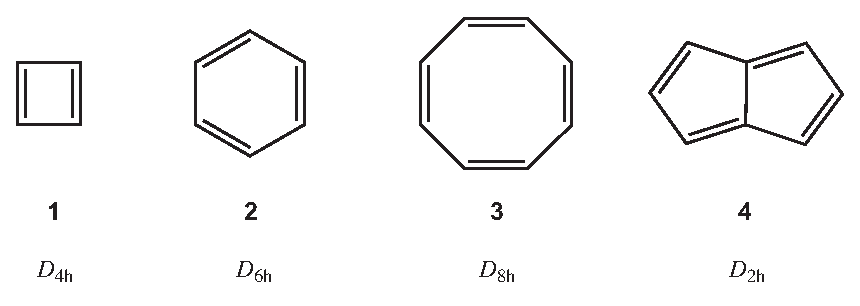
\includegraphics[scale=0.85]{orbopt/figures/compounds.eps}
\caption{Cyclobutadiene (\textbf{1}), benzene (\textbf{2}), cyclooctatetraene (\textbf{3}) and pentalene (\textbf{4}). Underneath the compound numbers the symmetry used for the respective compounds has been printed.}
\label{ch2.fig.compounds}
\end{figure}

Prior to any VB calculation, the geometry of the compounds had been optimized in the symmetry indicated in Figure \ref{ch2.fig.compounds}, using Restricted Hartree-Fock (RHF) with the \mbox{6-31G} basis set \cite{631g1,631g2}. The Valence Bond calculations, three per molecule, using the \textit{superci}, \textit{pert} and \textit{fock} options, were performed using delocalized $\sigma$ orbitals and strictly atomic $\pi$ orbitals, generated by a RHF calculation and an atomic SCF, respectively, all in the 6-31G basis. For all VB calculations, the DIIS option was switched on from the start. TURTLE's \textit{hybrid} option was used to separate the $\pi$ orbitals from each other and the $\sigma$ core. \textit{All} excitations were treated with perturbation, both for \textit{pert} and for \textit{fock}. In this case the \textit{fock} option can be used for the doubly occupied orbitals in the $\sigma$ core, because of the orthogonality of the $\pi$ orbitals to the $\sigma$ core. 

In Table \ref{ch2.tab.flat1} and \ref{ch2.tab.flat2} the results are presented. The total energies, presented below the name of each compound in the tables, was equal for all optimization methods for the first eight decimal places. Beneath the energies, for all methods the number of iterations, the total timings and the speed-up factors compared to regular Super CI are presented. In the case of the \textit{fock} option only the orbitals from the $\sigma$ core are optimized using the Fock algorithm; the $\pi$ orbitals are optimized using the \textit{pert} option in that case.

\begin{table}[htbp]
\caption{Below their names, the total energy of both molecules is presented. The number of iterations, timing per iteration and speed-up factors (compared to \textit{superci}) for butadiene and benzene.}
\begin{center}
\begin{tabular}{l c c c c c c}
\hline
&\multicolumn{3}{c}{\textbf{Butadiene}}&\multicolumn{3}{c}{\textbf{Benzene}}\\
&\multicolumn{3}{c}{(-153.59682368 au)}&\multicolumn{3}{c}{(-230.54408700 au)}\\
\textbf{Method}&\textbf{\# iter}&\textbf{sec/iter}&\textbf{speed-up}&\textbf{\# iter}&\textbf{sec/iter}&\textbf{speed-up}\\
\hline
\textit{superci}&8&73.0&1&8&2274.1&1\\
\textit{pert}&14&4.9&8&13&90.8&15\\
\textit{fock}&10&4.8&12&10&79.3&23\\
\end{tabular}
\label{ch2.tab.flat1}
\end{center}
\end{table}

\begin{table}[htbp]
\caption{Below their names, the total energy of both molecules is presented. The number of iterations, timing per iteration and speed-up factors (compared to \textit{superci}) for cyclooctatetraene and pentalene.}
\begin{center}
\begin{tabular}{l c c c c c c}
\hline
&\multicolumn{3}{c}{\textbf{Cyclooctatetraene}}&\multicolumn{3}{c}{\textbf{Pentalene}}\\
&\multicolumn{3}{c}{(-307.35606250 au)}&\multicolumn{3}{c}{(-306.14034868 au)}\\
\textbf{Method}&\textbf{\# iter}&\textbf{sec/iter}&\textbf{speed-up}&\textbf{\# iter}&\textbf{sec/iter}&\textbf{speed-up}\\
\hline
\textit{superci}&8&320106.0&1&8&47692.8&1\\
\textit{pert}&13&4704.2&42&14&1982.4&14\\
\textit{fock}&10&3857.0&66&12&1386.8&23\\
\end{tabular}
\label{ch2.tab.flat2}
\end{center}
\end{table}

For all molecules, the Super CI calculations take 8 iterations. Both in the \textit{fock} and in the \textit{pert} calculations more iterations are necessary to reach convergence. The approximation of the diagonal matrix element (Section \ref{ch2.sec.denominator}) seems to be beneficial for the calculation, because the number of iterations for \textit{fock} is smaller than for \textit{pert} in all four situations.

From the timings, it becomes clear that the \textit{fock} option is fruitful for this type of molecule, because the speed-up lies between 12 times for butadiene to 66 times for cyclooctatetraene compared to traditional Super CI. The difference between the speed-up of \textit{fock} and \textit{pert} is reasonable, but not as impressive as the difference between \textit{pert} and \textit{superci}. A drawback of the \textit{fock} option is the orthogonality condition that has to be met. 

Delocal VBSCF calculations, for which no examples have been presented here, do not suffer from this drawback, because in those calculations the doubly occupied orbitals will be orthogonal to each other, to the variably occupied orbitals and to the virtuals. However, most VB calculations in this thesis have been run with the \textit{hybrid} option, for which the \textit{fock} option is restricted to special cases, where the different \textit{hybrids} are orthogonal by symmetry.

% Not here, zegt Joop :
%The \textit{pert} option is more generally applicable, although in some cases, like in the first example, convergence aids are necessary to make the calculations converge, as seen before.

\section{Conclusions}

Fock matrix elements, which can be calculated faster than Brillouin matrix elements, can be used for all excitations for which the orbital from which the excitation takes place (usually the doubly occupieds) and the orbital to which the excitation is, are orthogonal to each other and to the other orbitals. The other orbitals are allowed to be non-orthogonal to one another. In combination with the \textit{hybrid} option the \textit{fock} option can only be used when the doubly occupied orbitals in different \textit{hybrids} are orthogonal to all other orbitals.

When Fock matrix elements can be used, the calculation takes less time with the \textit{fock} than with the \textit{pert} option. However, the difference between \textit{fock} and \textit{pert} is not as impressive as the difference between \textit{pert} or \textit{fock} and \textit{superci}. Furthermore, the \textit{fock} option is not as generally applicable as the \textit{pert} option, because the latter does not require any orthogonality amongst the orbitals.

\section{Outlook}

A drawback of the current implementation of the \textit{pert} and \textit{fock} options is that they are not automatic. A first extension would be the implementation of an automatic \textit{pert}/\textit{fock} option. For each excitation only the first column element and the diagonal element, \textit{e.g.} $\left < \Psi_{0} | \mathbf{H} - E_0 | \Psi_{ia} \right >$ and $\left < \Psi_{ia} | \mathbf{H} - E_0 | \Psi_{ia} \right >$, are calculated. With these two elements the orbital update coefficient $b_{ia}$ is calculated. Only when its absolute value is above a predefined threshold the other Brillouin matrix elements for the excitation are calculated. For small update coefficients the \textit{pert} (or \textit{fock} if the situation permits it) option is then automatically used, since no other Brillouin matrix elements are calculated. 

Another step towards an automatic \textit{pert}/\textit{fock} option would be the use of orbital energies. Orbitals, like core $\sigma$ orbitals have a low energy ($i$ in Figure \ref{ch2.fig.energy}). %
% Helaas een newpage, want anders komt plaatje tussen referenties.
% (toch weer niet)
%\clearpage
%\newpage
%
\begin{figure}[ht]
\center
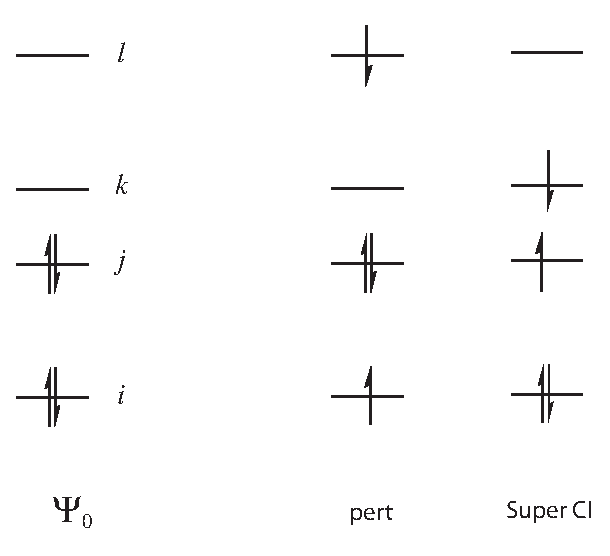
\includegraphics[width=2.8in]{orbopt/figures/orbitals.eps}
\caption{A wave function ($\Psi_0$), with two doubly occupied orbitals, one low lying ($i$) and one high lying ($j$). There are two virtual orbitals, one low lying ($k$) and one high lying ($l$). The excitation from $i$ to $l$ should be treated with the \textit{pert} option, while the excitation from $j$ to $k$ should be treated with regular Super CI.}
\label{ch2.fig.energy}
\end{figure} 
Excitations from these low lying orbitals to high lying virtuals ($l$) will only slightly change the wave function. Therefore, these orbitals  could easily be optimized by \textit{pert} or \textit{fock}. The HOMO-LUMO range ($j$, $k$), can be optimized by Super CI, since these orbitals are expected to change more than core orbitals. For the orbital energies the eigenvalues of a one electron operator on MO basis could be used.  Although these values are  estimates (interaction between orbitals is not taken into account), they can probably be used to separate between the excitations to be treated with the \textit{superci} and the \textit{pert} or \textit{fock} option. 

The use of the \textit{fock} option in combination with the \textit{hybrid} option may be used at this moment. However, it is assumed that the user will only use this combination when the doubly occupied orbitals in different \textit{hybrids} are orthogonal. An automatic orthogonality check for doubly occupied orbitals from different \textit{hybrids} would be desirable. In case of non-orthogonality, TURTLE should automatically use \textit{pert} instead of \textit{fock}. 

\section*{Appendix A: Cofactors}

A cofactor is a signed minor \cite{aitken}. A minor is created by removing one or more rows and columns from a determinant. Minors have the same sign as the original determinant from which they are derived. For a cofactor the sign depends on the position of the deleted row and column \cite{fokkeproef}. In this chapter the orbital overlap determinant, from which no rows and columns are removed, will be referred to as zeroth order cofactor. For a first order cofactor, obtained by removing one row and one column from the original determinant, the sign is $-1^{x+y}$, in which $x$ and $y$ are the indexes of the deleted row and column. For a second order cofactor, obtained by removing two rows and two columns from the original determinant, the sign is $-1^{x_1+x_2+y_1+y_2}$, in which $x_1$, $x_2$, $y_1$ and $y_2$ are the indexes of the deleted rows and columns. 

The overlap between two determinants can be expressed as  a zeroth order cofactor. The overlap of $\Delta_{1} = |ijkl \cdots n|$ with $\Delta_{2} = |ajkl \cdots n|$ for normalized orbitals is, \textit{e.g.}:
\begin{equation}
S_{12}^{(0)}=
\begin{array}{lllllll}
 &  i & j & k & l & \cdots & n \\
 a &  \multicolumn{1}{|l}{s_{ia}} & s_{ja}  & s_{ka} & s_{la} & & \multicolumn{1}{l|}{ s_{na} } \\
 j & \multicolumn{1}{|l}{s_{ij}} & 1 & s_{kj} & s_{lj} & & \multicolumn{1}{l|}{s_{nj}} \\
 k & \multicolumn{1}{|l}{s_{ik}} & s_{jk} & 1 & s_{lk} & & \multicolumn{1}{l|}{s_{nk}} \\
 l & \multicolumn{1}{|l}{s_{il}} & s_{jl} & s_{kl} & 1 & & \multicolumn{1}{l|}{s_{nl}} \\
 \vdots & \multicolumn{1}{|l}{ } &   &   & & \ddots & \multicolumn{1}{l|}{\vdots} \\
 n & \multicolumn{1}{|l}{ s_{in}} & s_{jn} & s_{kn} & s_{ln} & \cdots & \multicolumn{1}{l|}{1}
\end{array},\\
\label{ch2.eq.zocofac}
\end{equation}
in which the $s_{xy}$ elements stand for the orbital overlaps, \textit{i.e.} $\left < x | y \right >$. Along the rows and columns orbital labels are shown for readability. In the notation $S_{12}^{(0)}$, the superscript $(0)$ indicates that this is a zeroth order cofactor. The subscript $12$ indicates that the cofactor is constructed from overlaps of orbitals in determinant $\Delta_1$ with those from determinant $\Delta_2$.

A first order cofactor is derived from the zeroth order cofactor by removing one row and one column. So, when the column labeled $i$ and the row labeled $a$ are removed, the first order cofactor $S_{12}^{(i,a)}$ emerges:
\begin{equation}
S_{12}^{(i,a)} =
\begin{array}{lllllll}
 &  \hskip 2.0 pt \hbox{\lower 120pt\hbox{\vrule height128pt width 1.0pt}}\hskip-3.0pt i & j & k & l & \cdots & n \\
\noalign{\vskip-115pt}
 a &  \multicolumn{1}{|l}{s_{ia}} & s_{ja}  & s_{ka} & s_{la} & & \multicolumn{1}{l|}{ s_{na} } \\
\noalign{\vskip-8pt}
\multispan7\hbox{\vrule  height 1.0 pt width164pt}\cr
\noalign{\vskip 7pt}
  j & \multicolumn{1}{|l}{s_{ij}} & 1 & s_{kj} & s_{lj} & & \multicolumn{1}{l|}{s_{nj}} \\
 k & \multicolumn{1}{|l}{s_{ik}} & s_{jk} & 1 & s_{lk} & & \multicolumn{1}{l|}{s_{nk}} \\
 l & \multicolumn{1}{|l}{s_{il}} & s_{jl} & s_{kl} & 1 & & \multicolumn{1}{l|}{s_{nl}} \\
 \vdots & \multicolumn{1}{|l}{ } &   &   & & \ddots & \multicolumn{1}{l|}{\vdots} \\
 n & \multicolumn{1}{|l}{ s_{in}} & s_{jn} & s_{kn} & s_{ln} & \cdots & \multicolumn{1}{l|}{1}
\end{array}.\\
\label{ch2.eq.focofac}
\end{equation}
Since orbital $i$ is in the first column and orbital $a$ on the first row, the sign of the cofactor does not change because $-1^{(1+1)} = +1$.

When the columns labeled $i$ and $k$ and the rows labeled $a$ and $l$ are removed from $S_{12}^{(0)}$ the second order cofactor $S_{12}^{(i,k,a,l)}$ is generated:
\begin{equation}
S_{12}^{(i,k,a,l)} =
\begin{array}{lllllll}
 &  \hskip 2.0 pt \hbox{\lower 120pt\hbox{\vrule height128pt width 1.0pt}}\hskip-3.0pt i & j & \hskip 2.0 pt \hbox{\lower 120pt\hbox{\vrule height128pt width 1.0pt}}\hskip-3.0pt k & l & \cdots & n \\
\noalign{\vskip-115pt}
 a &  \multicolumn{1}{|l}{s_{ia}} & s_{ja}  & s_{ka} & s_{la} & & \multicolumn{1}{l|}{ s_{na} } \\
 \noalign{\vskip-8pt}
\multispan7\hbox{\vrule  height 1.0 pt width164pt}\cr
\noalign{\vskip 7pt}
 j & \multicolumn{1}{|l}{s_{ij}} & 1 & s_{kj} & s_{lj} & & \multicolumn{1}{l|}{s_{nj}} \\
 k & \multicolumn{1}{|l}{s_{ik}} & s_{jk} & 1 & s_{lk} & & \multicolumn{1}{l|}{s_{nk}} \\
 l & \multicolumn{1}{|l}{s_{il}} & s_{jl} & s_{kl} & 1 & & \multicolumn{1}{l|}{s_{nl}} \\
 \noalign{\vskip-8pt}
\multispan7\hbox{\vrule  height 1.0 pt width164pt}\cr
\noalign{\vskip 7pt}
 \vdots & \multicolumn{1}{|l}{ } &   &   & & \ddots & \multicolumn{1}{l|}{\vdots} \\
 n & \multicolumn{1}{|l}{ s_{in}} & s_{jn} & s_{kn} & s_{ln} & \cdots & \multicolumn{1}{l|}{1}
\end{array}.\\
\label{ch2.eq.socofac}
\end{equation}
In this second order cofactor the sign changes, because the position of the orbitals is: $i$ in the first and $k$ in the third column, $a$ on the first and $l$ on the fourth row. This makes $-1^{(1+3+1+4)} = -1$.

\bibliography{orbopt}
\bibliographystyle{../main/achemso}
